\chapter{DESENVOLVIMENTO}
Nesta seção, será descrito em detalhes cada etapa do desenvolvimento do sistema de aquisição e processamento de sinais. 

Com finalidade de detalhar o funcionamento, podemos observar na Figura 1, o fluxo seguido pelo sistema desenvolvido.

\begin{figure}[h] 
	\begin{center} 
		\begin{center}
			\changecaptionwidth 
			\captionwidth{15.6cm} %posicionamento da legenda
			\caption{\label{fig_fot7}Fluxo do sistema de aquisição e processamento do sinal.}
			\fbox{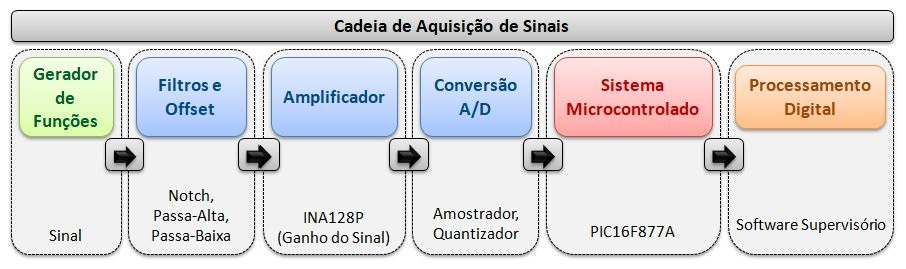
\includegraphics[scale=0.80]{figuras/fluxograma}}
			\fonte{adaptado de \cite{Geovani1}.}
		\end{center}
	\end{center}
\end{figure} 

 

\section{FILTROS ATIVOS}
O sinal é gerado com auxílio do gerador de funções, que inicia o processo passando pelo sistema de filtragem. Utilizando a Equação 4.1, calculou-se a frequência de corte dos filtros, possibilitando a escolha correta dos resistores e capacitores \cite{Geovani3}.

\begin{equation}
	fc = \frac {1}{2 \times \pi \times R \times C}
\end{equation}

Onde:
\begin{itemize}
	\item \textit{fc}: frequência de corte;
	\item \textit{R}: resistência ($\Omega$);
	\item \textit{C}: Capacitância (F).
\end{itemize}
 
Para o sistema de filtragem foi utilizado um filtro passa altas com frequência de corte em 0.5 Hz e um passa baixas com frequência de corte em 90 Hz. Aplicando a equação citada acima, os componentes resultantes para que os filtros funcionassem corretamente, podem ser visualizados no esquemático do circuito elétrico na Figura 2.

\begin{figure}[h] 
	\begin{center} 
		\begin{center}
			\changecaptionwidth 
			\captionwidth{15.8cm} %posicionamento da legenda
			\caption{\label{fig_fot7}Esquemático do circuito elétrico dos filtros do sinal}
			\fbox{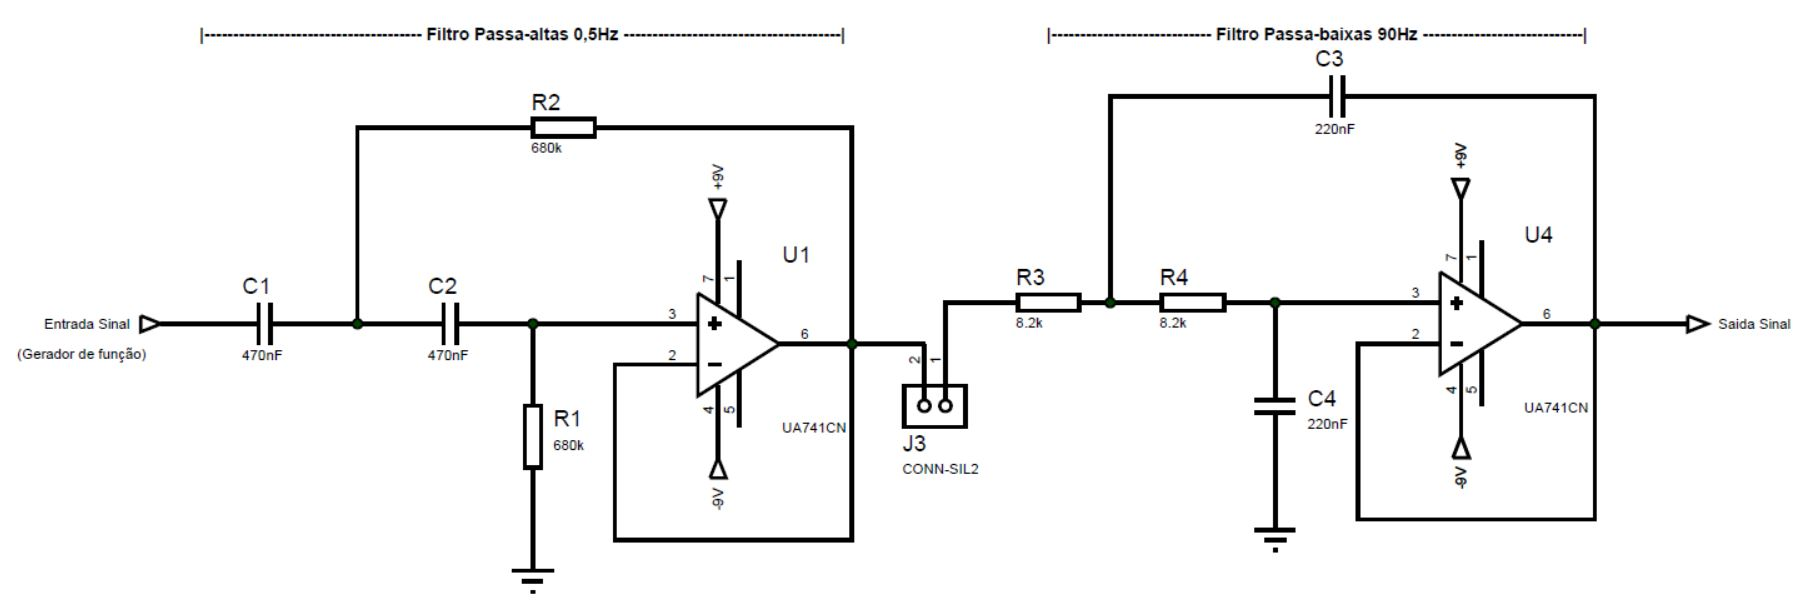
\includegraphics[scale=0.41]{figuras/circuitoFiltro}}
			\fonte{os autores.}
		\end{center}
	\end{center}
\end{figure} 

\section{AMPLIFICADOR}
Posteriormente à filtragem, para ser utilizado o sinal necessita ser amplificado. Diante isso, foi feito uso do amplificador de instrumentação INA128P. Neste componente, o valor de saída é definido pelo resistor de ganho, que é ligado aos pinos 1 e 8. Foi utilizado no desenvolvimento um resistor de 5.6k, obtendo uma amplificação de 10 vezes, de acordo com a fórmula de ganho apresentada na Equação 4.2 \cite{Geovani2}.  
\begin{equation}
	G = 1 + \frac {50k\Omega}{R_G}
\end{equation}

Onde:

\textit{G}: ganho;

\textit{R\tiny{G}}: resistor de ganho ($\Omega$).

A Figura 2 apresenta o circuito do amplificador. Onde R5 é o resistor de ganho, C5 e C6 são capacitores de 100nF para estabilizar a fonte do microcontrolador para não oscilar.
\newpage
\begin{figure}[h] 
	\begin{center} 
		\begin{center}
			\changecaptionwidth 
			\captionwidth{11.0cm} %posicionamento da legenda
			\caption{\label{fig_fot7}Esquemático do circuito elétrico do amplificador do sinal}
			\fbox{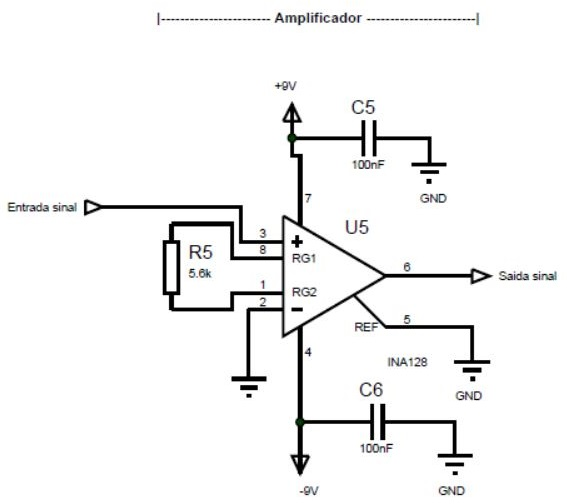
\includegraphics[scale=0.90]{figuras/circuitoAmplificador}}
			\fonte{os autores.}
		\end{center}
	\end{center}
\end{figure} 


\section{FIRMWARE}
Após filtrado e amplificado, o sinal precisa ser convertido de analógico para digital, este processo foi realizado com a utilização de um microcontrolador PIC 16F877A, pois possui um conversos A/D interno, tornando o processo simples. A Figura 4, demonstra o esquemático do circuito elétrico desenvolvido para tal processo. 

\begin{figure}[htb]
	\caption{Esquemático do circuito elétrico do sistema de conversão A/D}
	%	\label{diag:grafico6}
	\borda{
		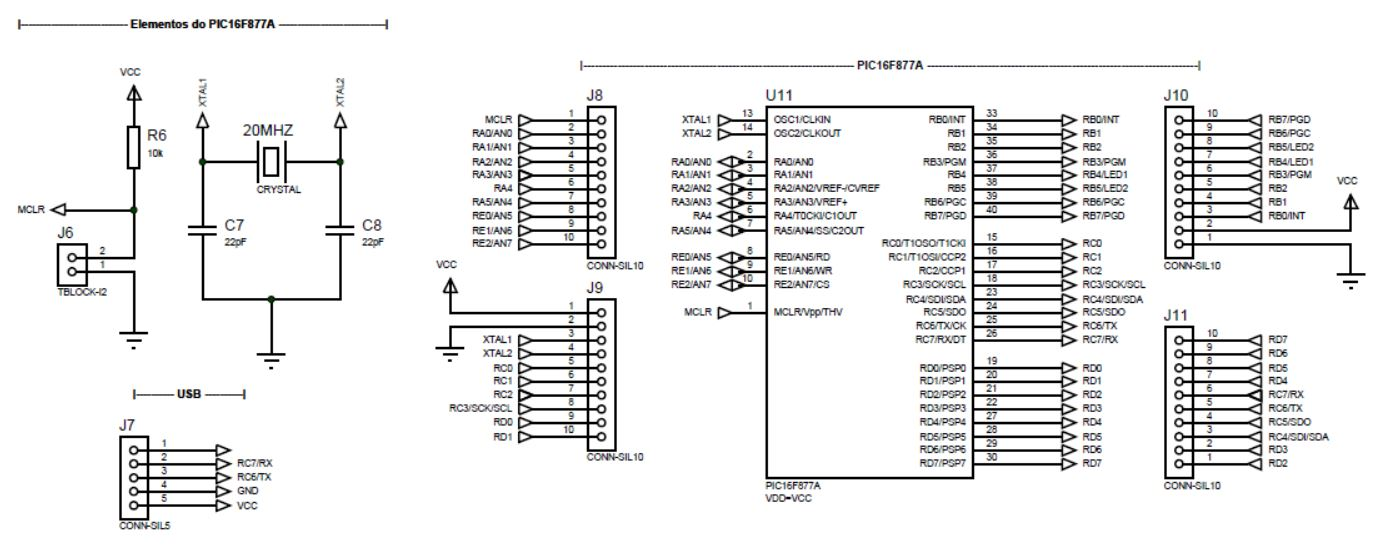
\includegraphics[scale=0.52]{figuras/circuitoPIC}
	}
	\fonte{os autores.}
\end{figure}

Posteriormente a conversão A/D do sinal, o mesmo é formatado com a utilização de colchetes para ser enviado so software supervisório. A leitura do sinal ocorre a cada 5 ms, onde são coletadas 200 amostras a cada período de leitura.

O código fonte do firmware pode ser consultado no Apêndice A.

\section{SOFTWARE}
Para o desenvolvimento do software supervisório, foi utilizado o software Qt Creator. A Figura 5, demonstra a tela inicial, que faz a leitura dos dados, através do botão "Ler Dados", no botão "Apresentar Gráfico" é possível visualizar a entrada do sinal, bem como manipulá-lo através do botão "Calcular DFT" e "Apresentar DFT".  Fazendo o uso de um período de mil amostras, é possível analisar o sinal através de uma DFT (Discrete Fourier Transform). 

\begin{figure}[htb]
	\caption{Software supervisório}
	%	\label{diag:grafico6}
	\borda{
		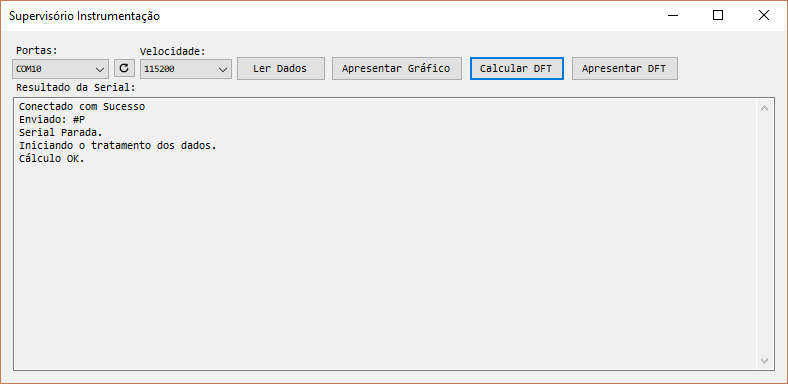
\includegraphics[scale=0.54]{figuras/software}
	}
	\fonte{os autores.}
\end{figure}

O código fonte de software supervisório desenvolvido pode ser verificado no Apêndice B.

\section{SISTEMA DE INSTRUMENTAÇÃO E PROCESSAMENTO DE SINAIS}
Após o detalhamento de cada módulo comentado nas seções anteriores, a Figura 6 demonstra o esquemático completo do hardware.

\begin{figure}[htb]
	\caption{Esquemático do circuito elétrico do sistema de instrumentação e processamento de sinais}
	%	\label{diag:grafico6}
	\borda{
		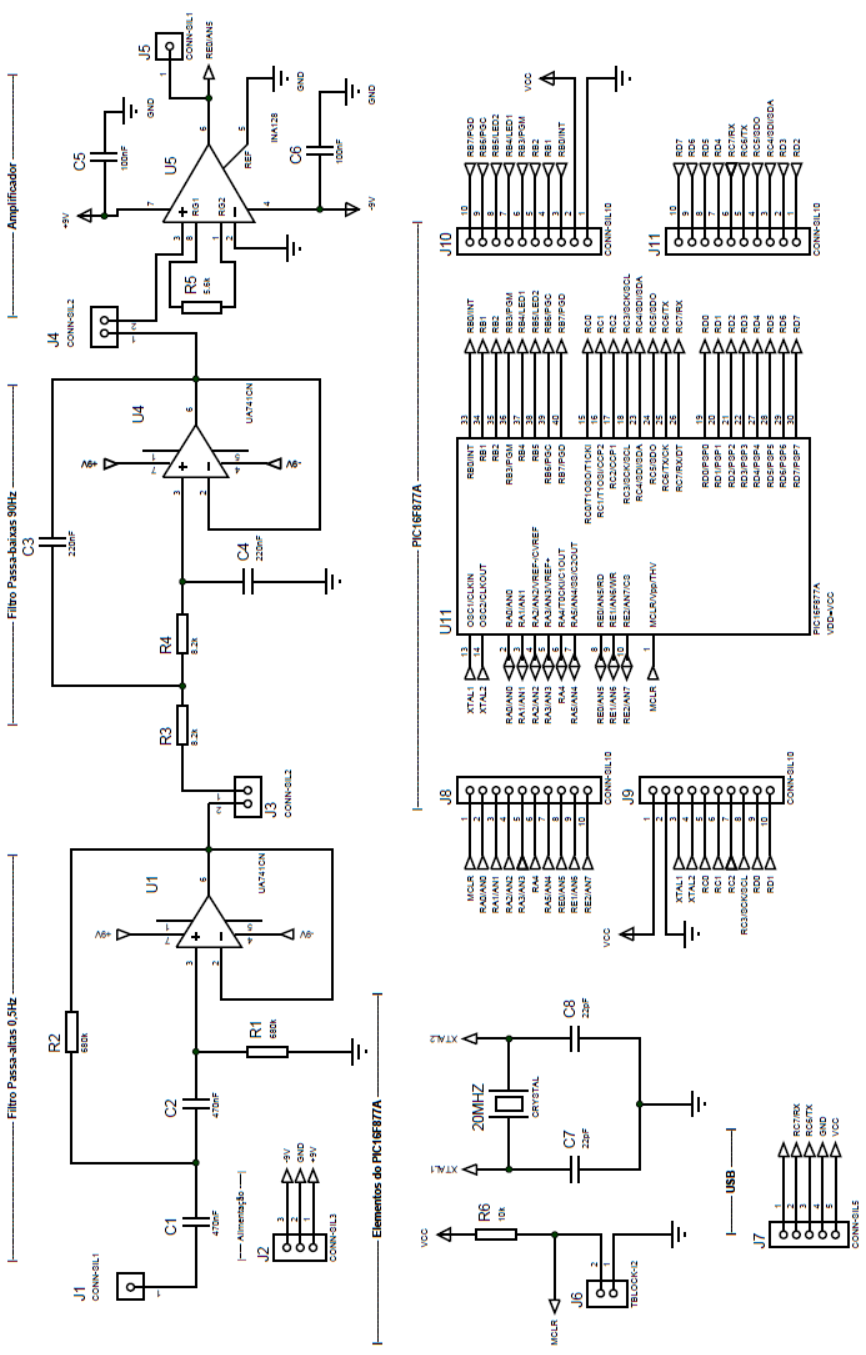
\includegraphics[scale=0.83]{figuras/completo}
	}
	\fonte{os autores.}
\end{figure}
